\documentclass[a4paper,11pt]{article}

% Packages
\usepackage[utf8]{inputenc}
\usepackage[T1]{fontenc}
\usepackage[french]{babel}
\usepackage{fancyhdr}
\usepackage{geometry}
\usepackage{amsmath}
\usepackage{amssymb}
\usepackage{algorithm}
\usepackage{algpseudocode}
\usepackage{graphicx}
\usepackage{listings}
\usepackage{xcolor}
\usepackage{forest}

% Page layout
\geometry{a4paper, margin=2.5cm}

% Fix header height issue
\setlength{\headheight}{14pt}

\lstset{
  backgroundcolor=\color{gray!10},
  basicstyle=\ttfamily\small,
  frame=single,
  breaklines=true,
  tabsize=2,
  showstringspaces=false,
  language=Java
}

% Header and footer setup
\pagestyle{fancy}
\fancyhf{}

% Header
\fancyhead[R]{ISIMA-POO}

% Footer
\fancyfoot[L]{Erkin Tunc Boya}
\fancyfoot[C]{Université de Clermont Auvergne}
\fancyfoot[R]{\thepage}

% Optional header/footer lines
\renewcommand{\headrulewidth}{0.4pt}
\renewcommand{\footrulewidth}{0.4pt}

% For demonstration of terminal tree
\lstdefinestyle{tree}{
  literate=
    {├}{{\textbar}}1
    {─}{{-}}1
    {└}{{+}}1
    {│}{{\textbar}}1
}

\begin{document}

\begin{center}
\Huge{Projet Gomoku}\\[0.5cm]
\Large{Erkin Tunc Boya}\\[0.2cm]
\Large{Mai-Avril 2025}
\end{center}

\section{Structure du Projet}

Pour organiser notre travail, on a opté pour une architecture en plusieurs dossiers, chacun ayant un rôle assez précis. Voici un rapide tour d'horizon :

\begin{itemize}
    \item \textbf{app/} : C'est ici que tout commence. Ce dossier s'occupe de coordonner le déroulement du jeu : mise en place de la partie, affichage terminal, appels aux fonctions de sauvegarde, etc. Un peu le "chef d'orchestre" du projet.
    \item \textbf{model/} : Ici, on trouve les classes qui décrivent le cœur du jeu : la grille, les jetons, les joueurs... et surtout la façon dont tout ce petit monde interagit entre eux.
    \item \textbf{ai/} : Ce dossier contient tout ce qui touche à l'intelligence artificielle. Rien de très poussé, mais suffisant pour donner un peu de fil à retordre au joueur humain.
    \item \textbf{save/} : Les fonctions qui permettent d'enregistrer ou de reprendre une partie en cours. On s'appuie sur la sérialisation pour garder l'état du jeu.
    \item \textbf{util/} : Quelques utilitaires pratiques pour améliorer l'affichage en console, notamment pour gérer les couleurs et les styles.
\end{itemize}

On a essayé de garder une organisation simple et cohérente, pour s'y retrouver facilement même après plusieurs jours sans toucher au code.

\section{Fonctionnalit\'es du Projet}

Notre version de Gomoku propose plusieurs options sympa :

\begin{itemize}
    \item Grille dynamique qui peut s'agrandir si besoin.
    \item V\'erification efficace des alignements (lignes, colonnes, diagonales).
    \item Joueur contre IA de base.
    \item Sauvegarde et reprise de partie.
    \item Interface terminal avec des couleurs pour plus de clart\'e.
    \item Possibilit\'e de personnaliser la taille de la grille et le nombre de pions \`a aligner.
\end{itemize}

\section{Comment Compiler et Exécuter}

Pour compiler et lancer le jeu, deux solutions \\
Utiliser directement les commandes classiques :
\begin{lstlisting}
javac -d target/classes src/main/java/*/*.java
java -cp target/classes app.Gomoku
\end{lstlisting}

Ou tout simplement passer par les scripts fournis :

\begin{itemize}
        \item \texttt{runGomoku.bat} pour Windows
        \item \texttt{runGomoku.sh} pour Linux ou Mac
    \end{itemize}

Ces scripts compilent automatiquement tous les fichiers sources et lancent le jeu.
\newpage

\section{G\'en\'eration de la Documentation}

La JavaDoc peut \^etre g\'en\'er\'ee via :
\begin{itemize}
    \item \texttt{generateDocs.bat} pour Windows
    \item \texttt{generateDocs.sh} pour Linux ou Mac
\end{itemize}
Cela cr\'eera une documentation HTML dans le dossier \texttt{/doc/}

Ces scripts créent une documentation HTML dans le dossier \texttt{/doc/}.

\section{Sauvegardes des Parties}

Les parties sauvegard\'ees se trouvent dans le dossier \texttt{/data/}, sous forme de fichiers \texttt{.dat}.

\vspace{15mm}
\section{Organisation Visuelle du Projet}

Voici l'organisation visuelle des dossiers et fichiers du projet :

\begin{lstlisting}[style=tree]
Gomoku-Game-Projet/
├── Gomoku/
│   ├── generateDocs.bat         # Windows : Generer JavaDoc
│   ├── generateDocs.sh          # Linux/Mac : Generer JavaDoc
│   ├── runGomoku.bat            # Windows : Compiler et executer Gomoku
│   ├── runGomoku.sh             # Linux/Mac : Compiler et executer Gomoku
│   ├── data/                    # Sauvegardes des parties
│   │   └── ErkinVsAI.dat
│   ├── src/
│   │   ├── main/
│   │   │   └── java/
│   │   │       ├── ai/           # Logique de l'IA
│   │   │       ├── app/          # Application principale
│   │   │       │   └── Gomoku.java
│   │   │       ├── model/        # Modeles du jeu
│   │   │       ├── save/         # Gestion sauvegarde/chargement
│   │   │       └── util/         # Utilitaires
│   │   └── test/                 # Reserve aux tests
│   │       └── java/
│   └── target/
│       ├── classes/              # Fichiers .class compiles
│       └── test-classes/
├── rapport/                      # Rapport LaTeX
│   └── rapport.tex
├── README.md                      # Documentation
└── .gitignore                     # Regles Git
\end{lstlisting}

\newpage

\section{Diagramme UML}


Un diagramme UML pr\'esente les liens entre les classes principales du projet, notamment celles du \texttt{model/} et la classe \texttt{GameEngine} du dossier \texttt{app/}.


\begin{figure}[h!]
    \centering
    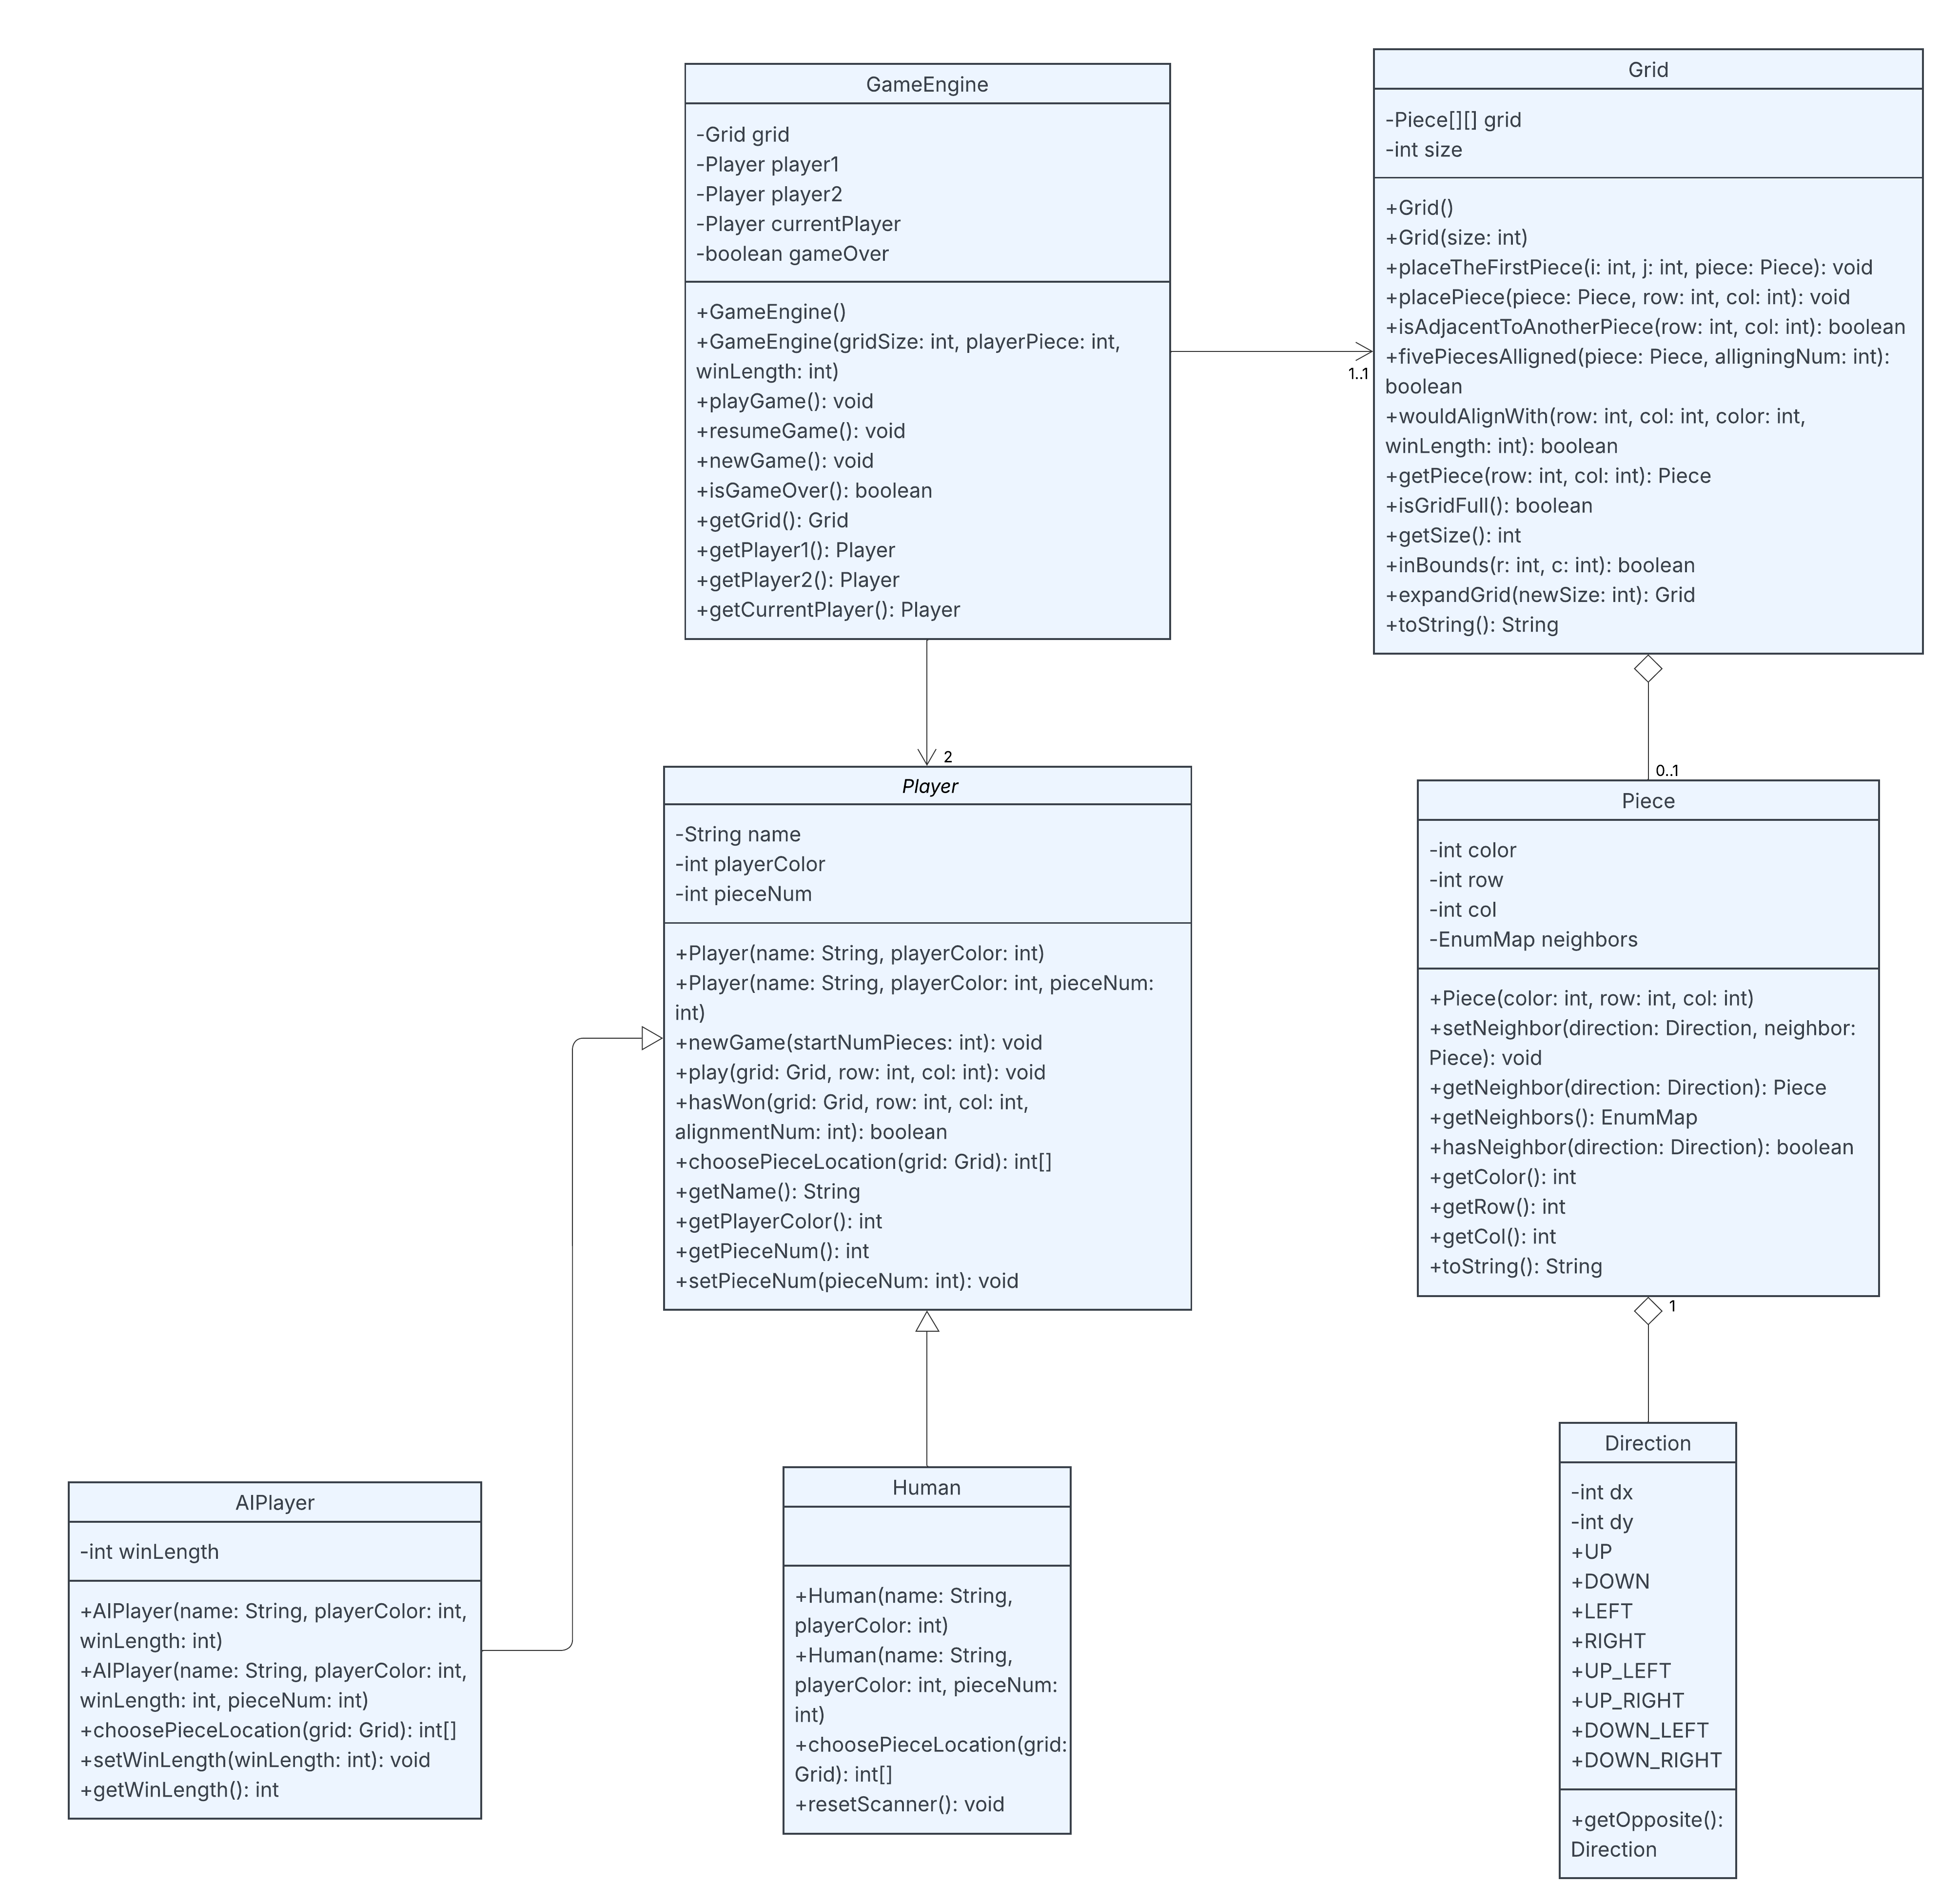
\includegraphics[width=1\textwidth]{img/gomoku-UML.png}
    \caption{Diagramme UML de la logique du projet Gomoku}
    \label{fig:uml}
\end{figure}

\end{document}
